\documentclass[margin=1mm]{standalone}
\usepackage{enumitem}
\usepackage[skip=3mm, indent=0mm]{parskip}
\usepackage{fontspec}
\setmainfont{QTHeidelbergType}

\usepackage[x11names]{xcolor}
\usepackage{tikz}
\colorlet{fascist}{OrangeRed1}
\colorlet{liberal}{Turquoise4}

\begin{document}
	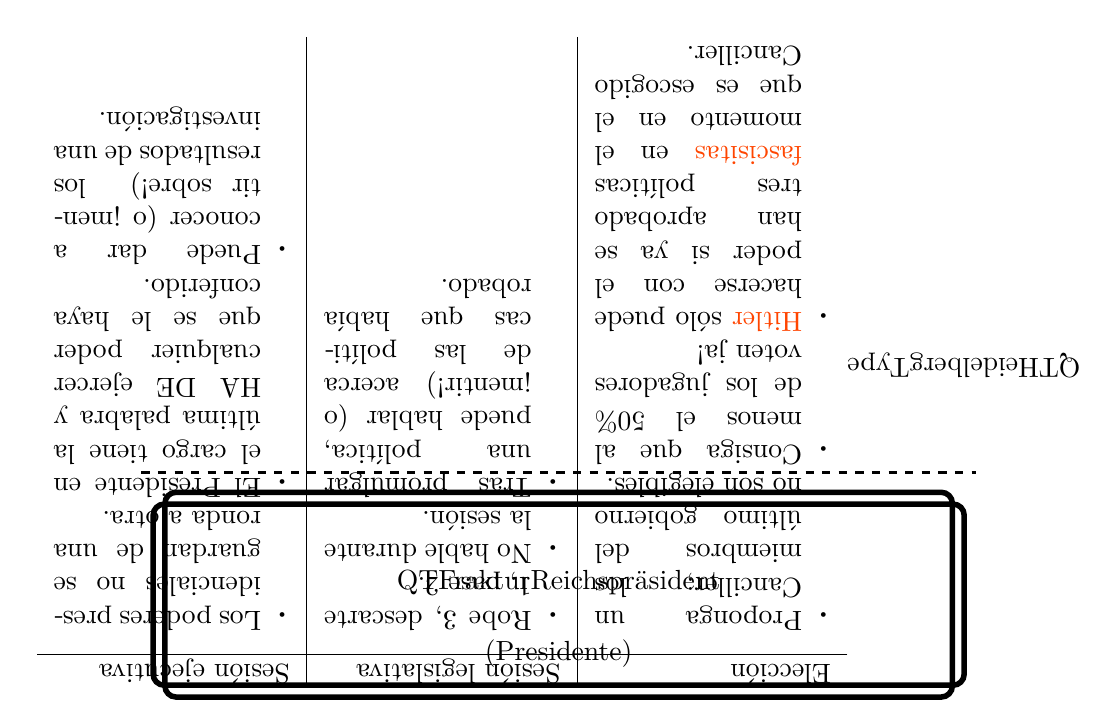
\begin{tikzpicture}		
		
		\node at (0,0) {\fontsize{40}{40}\setmainfont{QTFraktur}Reichspräsident};
		\node at (0,-0.9) {(Presidente)};
		
		\draw [line width=2, rounded corners] (-5.15,1) rectangle (5.15,-1.3);
		\draw [line width=2, rounded corners] (-5,1.15) rectangle (5,-1.45);
		
		\fill [white] (-5.3, 1.4) rectangle (5.3, 4.25);
		\draw [dashed, line width=1] (-5.3, 1.4)--(5.3, 1.4);
		%\draw (-5.3, 1.7) rectangle (5.3, 4);
		
		\begin{scope}[yshift=2.8cm]
			\node at (0,0) [rotate=180] {\fontsize{5.75}{5.75}\setmainfont{QTHeidelbergType}\begin{tabular}{p{3cm}|p{3cm}|p{3cm}}
				Elección & Sesión legislativa & Sesión ejecutiva\\
				\hline
				\begin{itemize}[leftmargin=*]
					\item Proponga un Canciller; los miembros del último gobierno no son elegibles.
					\item Consiga que al menos el 50\% de los jugadores voten ja!
					\item \textcolor{fascist}{Hitler} sólo puede hacerse con el poder si ya se han aprobado tres políticas \textcolor{fascist}{fascisitas} en el momento en el que es escogido Canciller.
				\end{itemize} & 
				\begin{itemize}[leftmargin=*]
					\item Robe 3, descarte 1, pase 2.
					\item No hable durante la sesión.
					\item Tras promulgar una política, puede hablar (o ¡mentir!) acerca de las políticas que había robado.
				\end{itemize} & 
				\begin{itemize}[leftmargin=*]
					\item Los poderes presidenciales no se guardan de una ronda a otra.
					\item El Presidente en el cargo tiene la última palabra y HA DE ejercer cualquier poder que se le haya conferido.
					\item Puede dar a conocer (o ¡mentir sobre!) los resultados de una investigación.
				\end{itemize} 
			\end{tabular}};
		\end{scope}
		
	\end{tikzpicture}
\end{document}